\begin{document}

{
    \usebackgroundtemplate{
\includegraphics[width=\paperwidth]{capa.png}}
    \begin{frame}[plain]
        \vspace{18mm}
        \begin{flushright}
        \textcolor{cinza}{\textbf{\large{\thetitle}}}
    \end{flushright}

    \vspace{-6mm}
    \begin{flushright}
        \textcolor{cinza}{\textbf{\scriptsize{\theauthor}}}
    \end{flushright}

    \vspace{-7mm}
    %%%
    %%% Formação | Departamento | Centro
    %%%
    \begin{flushright}
        \textcolor{cinza}{\scriptsize{
            Bacharelado em Ciência da Computação | Informática e Estatística | Centro Tecnológico
        }}
    \end{flushright}


    \end{frame}
}

%%%
%%% Demais slides (exceto o slide final)
%%%
\begin{frame}{Terminologia}
    \begin{itemize}
        \item \textbf{Busca:} Conceito genérico de busca;
        \item \textbf{Consulta:} Processo completo de buscar por processos;
        \item \textbf{Consulta Processual:} Preencher e enviar o formulário de
            consulta processual de um TJ.
    \end{itemize}
\end{frame}

\begin{frame}{Estrutura}
    \tableofcontents
\end{frame}

\section{TJScraper}

\begin{frame}{O que é}
    TJScraper é uma biblioteca e uma aplicação de \textbf{extração} de dados
    processuais de portais públicos dos Tribunais de Justiça Brasileiro.

    \vspace{1em}

    Interfaces:
    \begin{itemize}
        \item Linha de Comando (ILC);
        \item Web.
    \end{itemize}
\end{frame}

\begin{frame}{Organização Geral}
    \begin{figure}[H]
        \centering
        \begin{tikzpicture}[
                scale=0.6,
                transform shape,
                edge from parent path={(\tikzparentnode\tikzparentanchor) |- (\tikzchildnode\tikzchildanchor)},
                % Childs
                module/.style = {grow = down, anchor = west, xshift=1em,
                    edge from parent path={(\tikzparentnode.south) |- (\tikzchildnode.west)},
                },
                category/.style = {},
                % Categories
                level 1/.style = {sibling distance = 8em},
                level 2/.style = {level distance = 5em},
                interface/.style = {grow = down, rectangle, draw, blue, fill=blue!20},
                utils/.style = {grow = down, rectangle, draw, gray, fill=gray!20},
                extract/.style = {grow = down, rectangle, draw, green!50!black, fill=green!20},
            ]
            \node [draw] {tj\_scraper}
                child [grow=down] [edge from parent fork down]
                child [category] {
                    node[utils] {Utilitários}
                        child [module, level distance = 1 * 3em] {node [utils] {.errors}}
                        child [module, level distance = 2 * 3em] {node [utils] {.process}}
                        child [module, level distance = 3 * 3em] {node [utils] {.statistics}}
                        child [module, level distance = 4 * 3em] {node [utils] {.timing}}
                        child [module, level distance = 5 * 3em] {node [utils] {.url}}
                    }
                child [category] {
                    node[interface] {Interface}
                        child [module, level distance = 1 * 3em] {node [interface] {.cli}}
                        child [module, level distance = 2 * 3em] {node [interface] {.webapp}}
                    }
                %[edge from parent fork down]
                child [category] {
                    node[extract] {Extração}
                        child [module, level distance = 1 * 3em] {node [extract] {.cache}}
                        child [module, level distance = 2 * 3em] {node [extract] {.download}}
                        child [module, level distance = 3 * 3em] {node [extract] {.export}}
                        child [module, level distance = 4 * 3em] {node [extract] {.html}}
                    }
                ;
        \end{tikzpicture}
    \end{figure}
\end{frame}

\begin{frame}{ILC (Interface de Linha de Comando)}
    Aplicação criada via Typer voltada a \textbf{desenvolvedores}, organizada
    em comandos e subcomandos:

    \begin{itemize}
        \item \textbf{\texttt{cache}:} Executa operações relacionadas à
            \textit{cache} através de subcomandos.
        \item \textbf{\texttt{download}:} Executa uma consulta.
        \item \textbf{\texttt{export}:} Exporta o resultado de uma consulta
            anterior (formato JSONLines) para uma planilha XLSX.
        \item \textbf{\texttt{webapp}:} Inicializa a aplicação Web (para
            desenvolvimento). Opcional.
    \end{itemize}
\end{frame}

\begin{frame}{Aplicação Web}
    \begin{figure}[H]
        \centering
        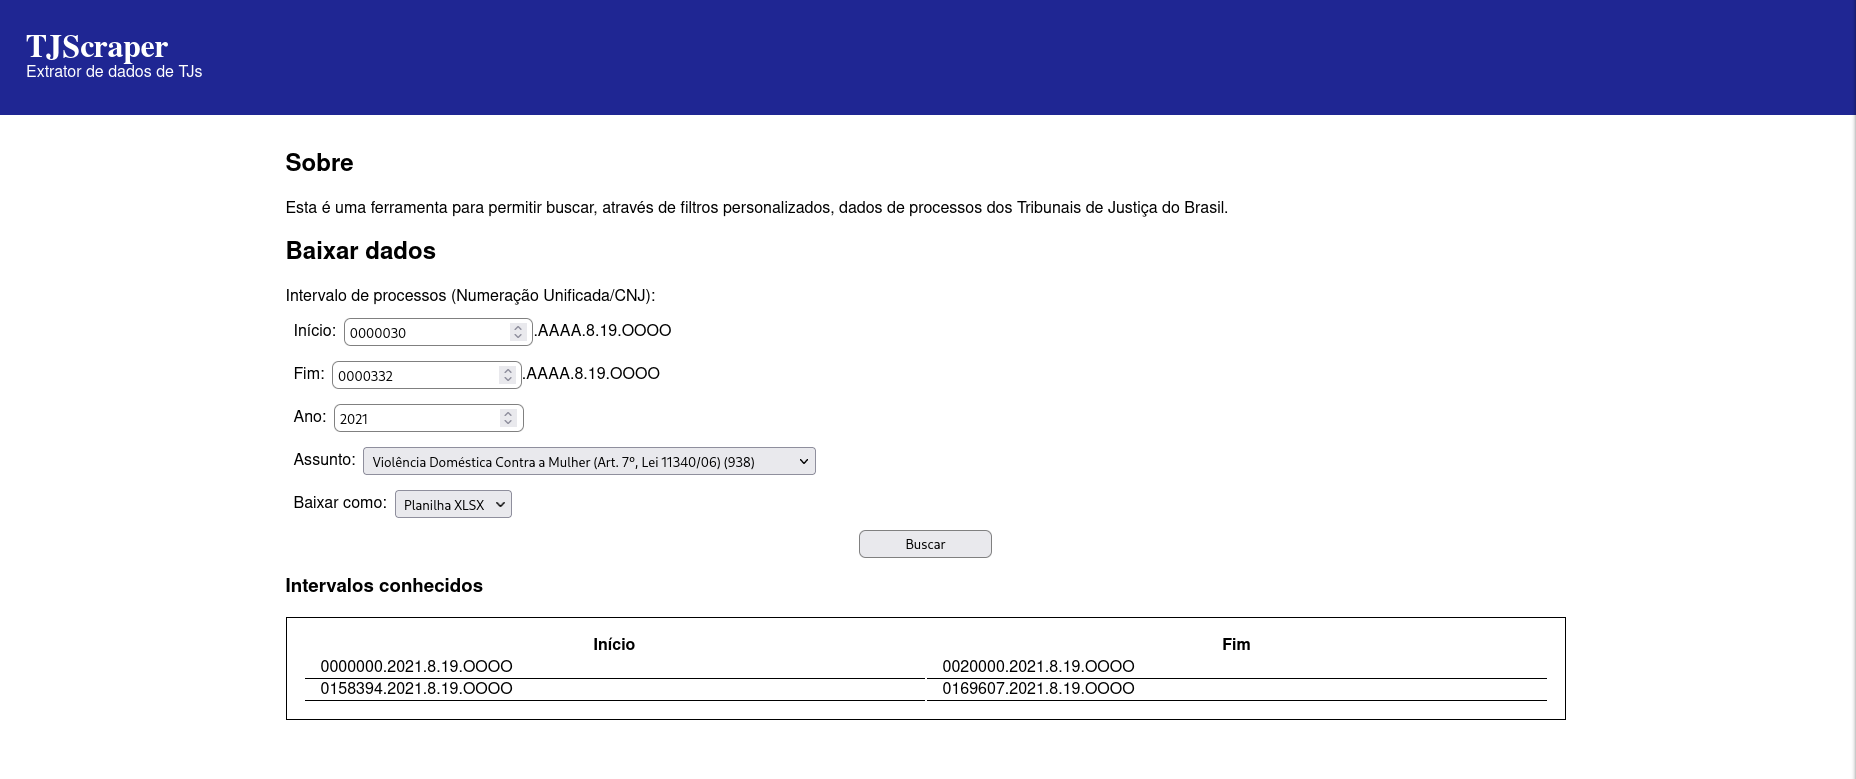
\includegraphics[keepaspectratio,width=1\textwidth]{img/tjscraper-webapp-1}
    \end{figure}
\end{frame}

\section{Estratégias de extração}

\subsection{Como descobrir processos}

\begin{frame}{TJ-RJ: Consulta Processual via ww4}
    \tiny Rota: \url{http://www4.tjrj.jus.br/ConsultaUnificada/consulta.do\#tabs-numero-indice0}.
    \begin{figure}[htb]
        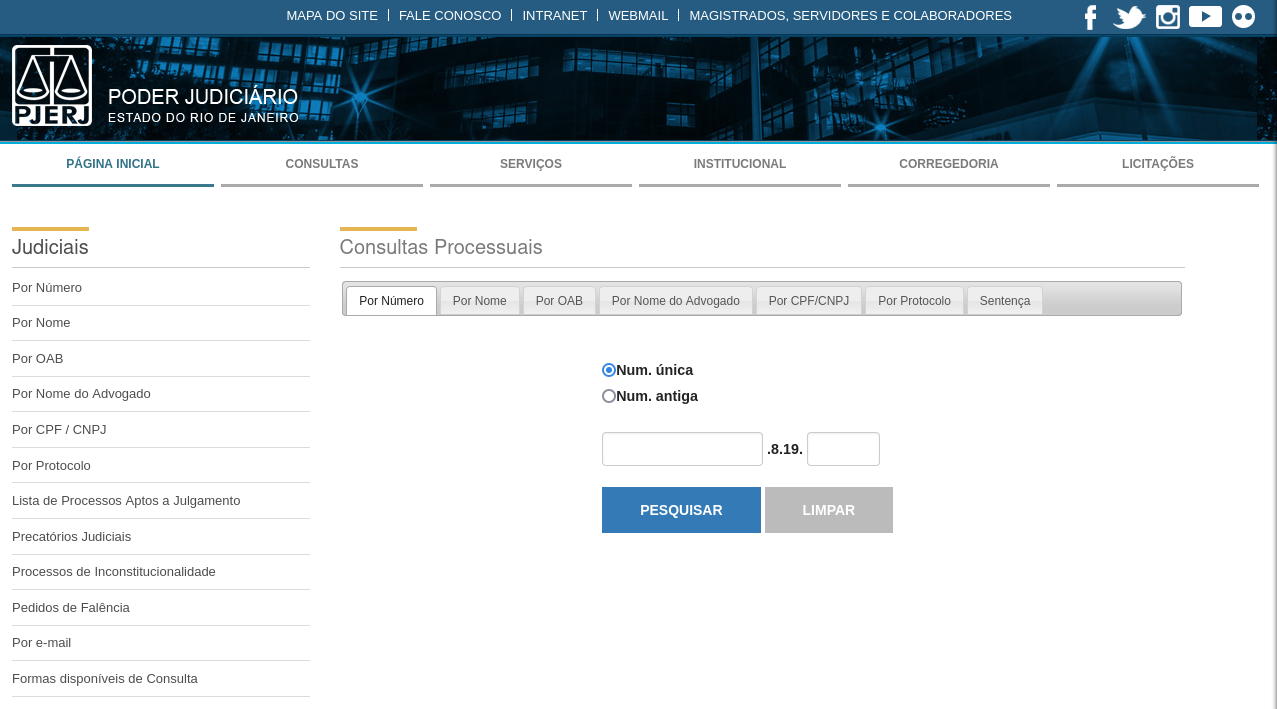
\includegraphics[keepaspectratio,width=1\textheight]{img/tj-rj-pagina-consulta}
    \end{figure}
\end{frame}

\begin{frame}{Sistemas de Numeração}
    \begin{itemize}
        \item \textbf{Unificada}: Padronizado pelo CNJ. Formato:
            ``NNNNNNN-DD.AAAA.J.TR.OOOO''.
        \item \textbf{Antiga}: Padrão interno de cada TJ. Formato do TJ-RJ:
            ``AAAA.OOO.NNNNNN-N''.
    \end{itemize}
\end{frame}

\begin{frame}{Exemplo de processo}
    Nº do processo: \textbf{2021.004.015548-9} (antiga).

    \begin{figure}[htb]
        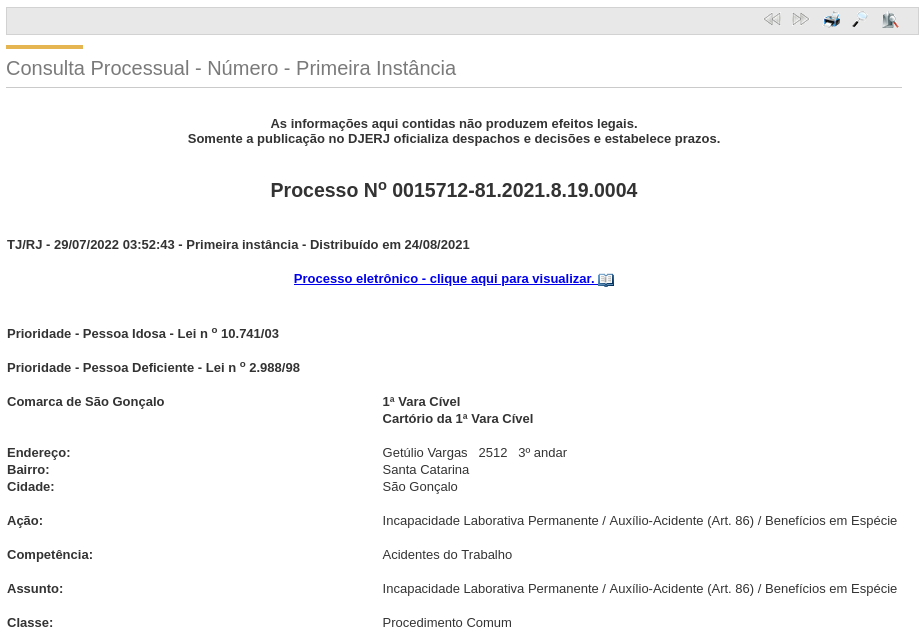
\includegraphics[keepaspectratio,width=0.8\textheight]{img/tj-rj-exemplo-de-processo}
    \end{figure}
\end{frame}

\begin{frame}{Numeração Unificada}
    \textcolor{blue}{0015712}-\textcolor{purple}{81}.\textcolor{red}{2021}.8.19.\textcolor{green!50!black}{0004}.

    \begin{itemize}
        \item \textcolor{blue}{0001000}: Número dado \textbf{sequencialmente};
        \item \textcolor{purple}{95}: $98 -1571220218190004 * 100 \mod 97 = 81$;
        \item \textcolor{red}{2021}: Ano de 2021;
        \item 8.19: Tribunal Regional Estadual do Rio de Janeiro;
        \item \textcolor{green!50!black}{0004}: Comarca de São Gonçalo.
    \end{itemize}

    \begin{figure}[H]
        \includegraphics[keepaspectratio]{img/tj-rj-comarca-sao-gonçalo}
    \end{figure}
\end{frame}

\begin{frame}{Numeração Antiga}
    \textcolor{red}{2021}.\textcolor{green!50!black}{004}.\textcolor{blue}{015548-9}.

    \begin{itemize}
        \item \textcolor{red}{2021}: Ano de 2021;
        \item \textcolor{green!50!black}{004}: Comarca de São Gonçalo.
        \item \textcolor{blue}{015548}: Número dado sequencialmente*;
        \item \textcolor{blue}{9}: Dígito verificador;
    \end{itemize}
\end{frame}

\subsection{Extração HTML}

\begin{frame}{TJ-RJ: Visualização de Processos}
    \begin{figure}[htb]
        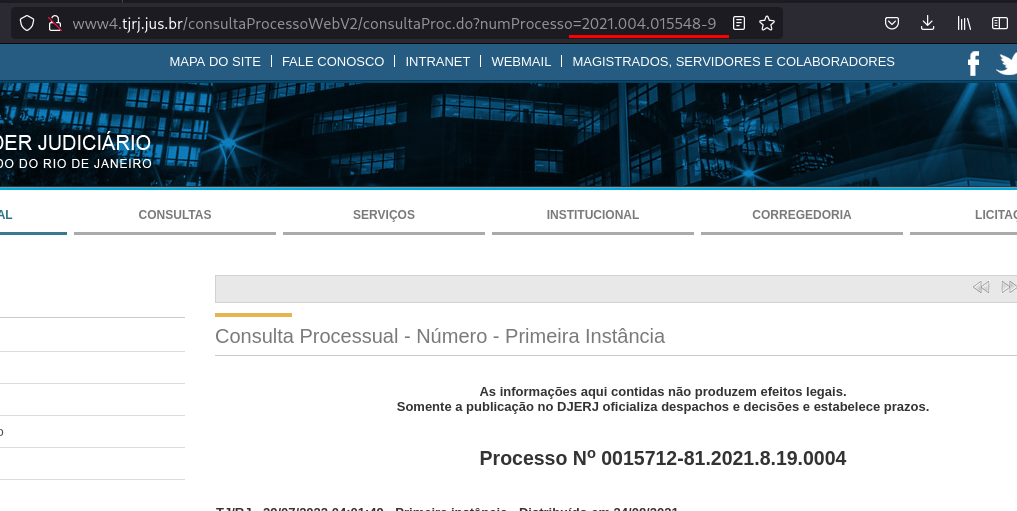
\includegraphics[keepaspectratio,width=1\textwidth]{img/tj-rj-1}
    \end{figure}
\end{frame}

\begin{frame}{TJ-RJ: Visualização de Processos}
    \begin{figure}[htb]
        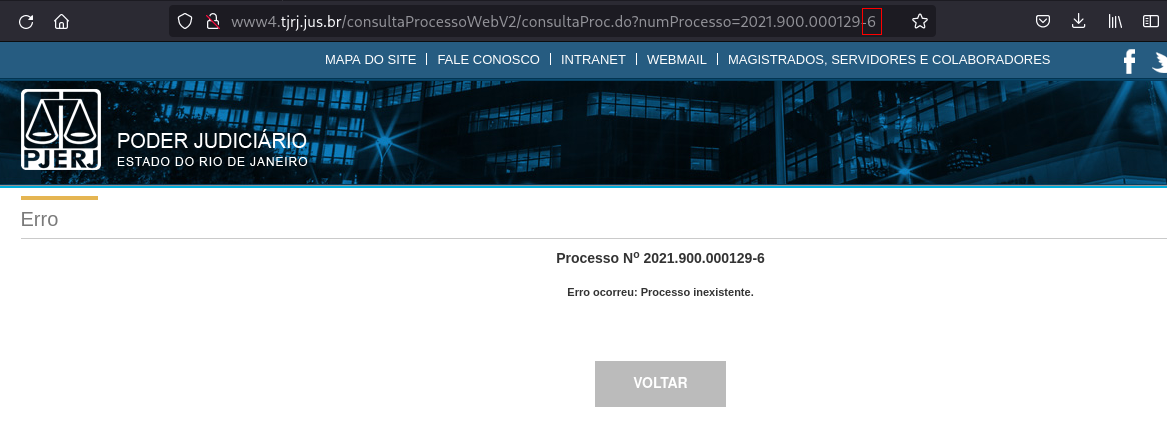
\includegraphics[keepaspectratio,width=1\textwidth]{img/tj-rj-2}
    \end{figure}
\end{frame}

\begin{frame}{Etapas}
    \begin{itemize}
        \item Descoberta e \textit{Download} de processos via numeração
            \textbf{antiga};
        \item \textit{Parsing} de HTML;
        \item Exportação de processos.
    \end{itemize}
\end{frame}

\begin{frame}{Scrapy e XPath}
    % Revisitaremos a escolha de Scrapy mais à frente nas conclusões

    \begin{tikzpicture}
    [
        every node/.append style = {anchor = west},
        grow via three points={one child at (0.5,-0.8) and two children at (0.5,-0.8) and (0.5,-1.6)},
        edge from parent path={(\tikzparentnode\tikzparentanchor) |- (\tikzchildnode\tikzchildanchor)},
        interface/.style = {rectangle, draw, blue, fill=blue!20},
        utils/.style = {rectangle, draw, gray, fill=gray!20},
        extract/.style = {rectangle, draw, green!50!black, fill=green!20},
    ]
        \node [extract] {tj\_scraper.html}
            child { node {\mintinline{python}{class TJRJSpider(Spider): ...}} }
            child {node {\mintinline{python}{def run_spider(spider, **kwargs)}}}
            child {node {\mintinline{python}{def extract_page_content(response)}}}
            child {node {\mintinline{python}{def extract_field(response, field_text)}}}
            child {node {\mintinline{python}{def check_for_captcha(response)}}}
            child {node {\mintinline{python}{def check_for_valid_id(response)}}}
        ;

    \end{tikzpicture}
\end{frame}


\begin{frame}[fragile]{HTML de um campo}
    \begin{minted}[gobble=4,breaklines]{html}
        <tr>
          <td class="info" valign="top" nowrap="nowrap">Assunto:</td>
          <td valign="top">
            Incapacidade Laborativa Permanente / Auxílio-Acidente (Art. 86) / Benefícios em Espécie
          </td>
        </tr>
    \end{minted}

    \vspace{1ex}

    XPath: \mintinline{text}{//td[text()='Assunto:']/following-sibling::td/text()}
\end{frame}

\begin{frame}{Detecção de páginas de erro}
    \begin{tabular}{ll}
        \toprule
        Erro & XPath \\
        \midrule
        Página de \textit{Captcha} & \mintinline{text}{//*[@id="container_captcha"]} \\
        Número inválido & \texttt{//title/text()} \\
        \bottomrule
    \end{tabular}
\end{frame}

\subsection{Extração via API JSON}

\begin{frame}{TJ-RJ: Consulta processual via ww3}
    % Colocar página de busca do ww3
    \tiny Rota: \url{https://www3.tjrj.jus.br/consultaprocessual/\#/consultapublica\#porNumero}.
    \begin{figure}
        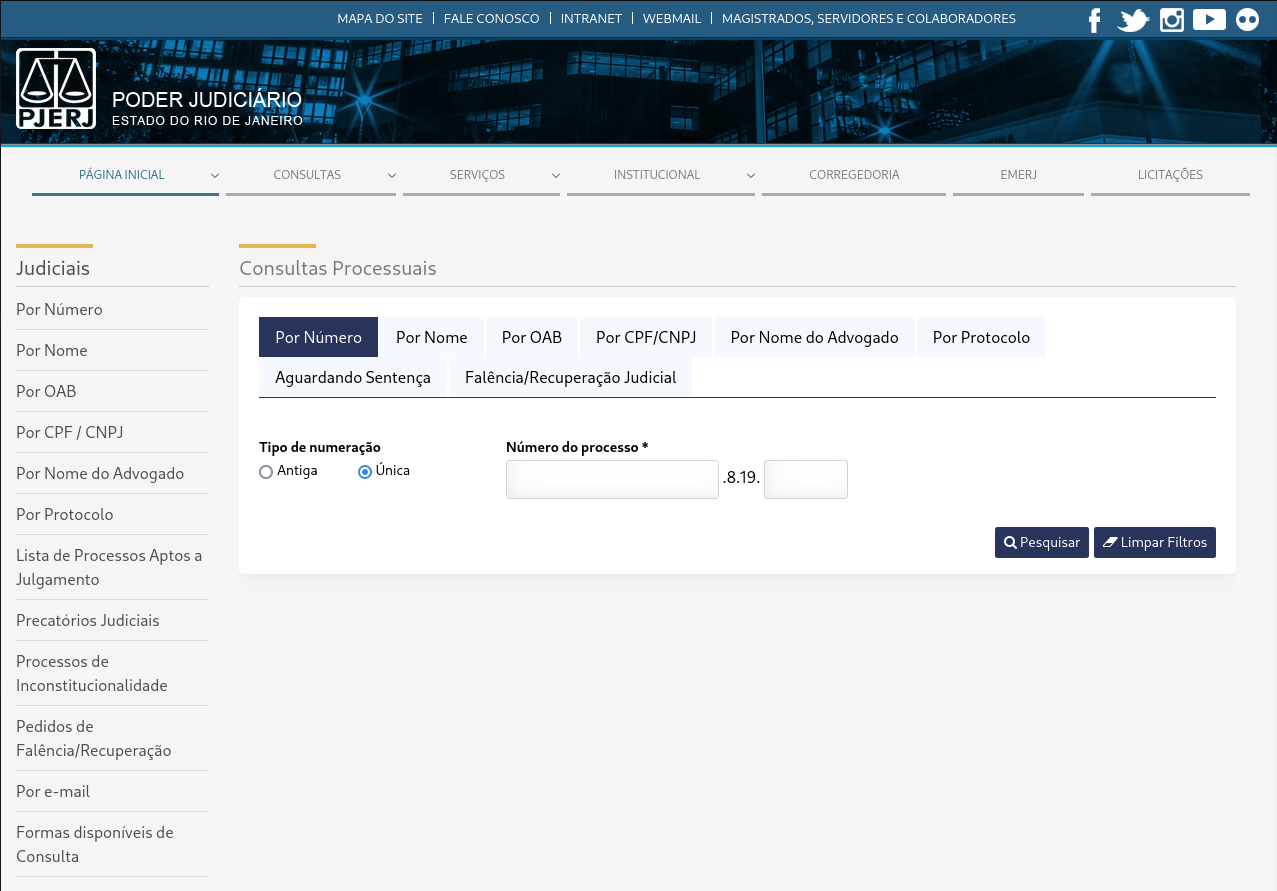
\includegraphics[keepaspectratio,width=0.9\textheight]{img/tj-rj-pagina-consulta-ww3}
    \end{figure}
\end{frame}

\begin{frame}{TJ-RJ: Consulta processual via ww3}
    % Colocar logs de Network do navegador
    \begin{figure}
        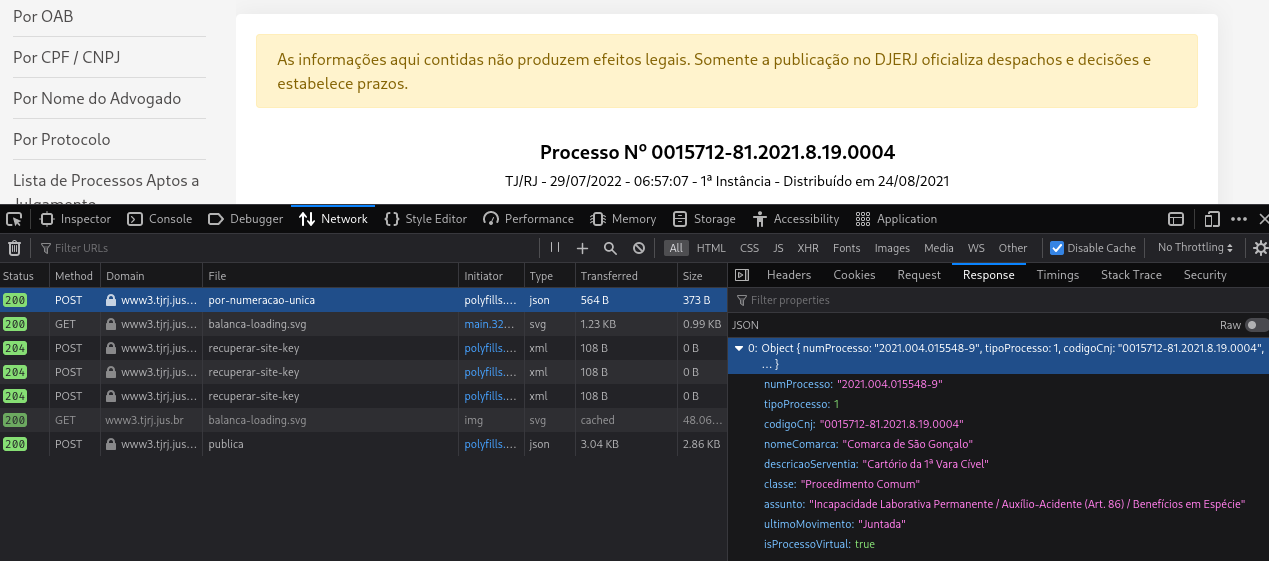
\includegraphics[keepaspectratio,width=1\textheight]{img/tj-rj-ww3-resposta-unica}
        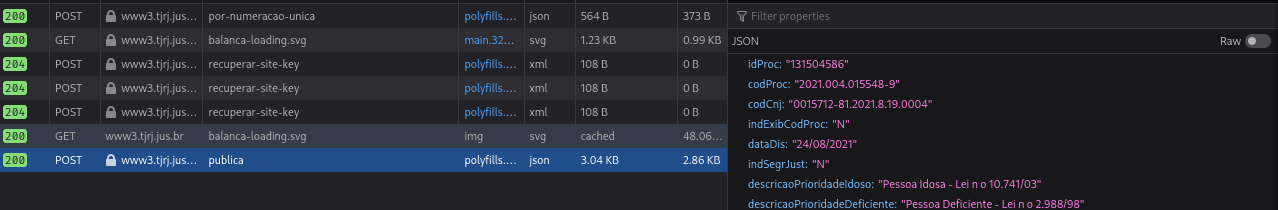
\includegraphics[keepaspectratio,width=1\textheight]{img/tj-rj-ww3-resposta-antiga}
    \end{figure}
\end{frame}

\begin{frame}{TJ-RJ: Objetos JSON}
    % Mostrar resposta para numeração única (pode ser print do navegador)
    % Mostrar resposta para numeração antiga (pode ser print do navegador)
    Parâmetros de URL: \texttt{tipoProcesso} e \texttt{codigoProcesso}.

    \vspace{1ex}

    Respostas de de erro:
    \begin{itemize}
        \tiny
        \item \mintinline{json}{["O processo informado não foi encontrado."]}
        \item \mintinline{json}{["Número do processo inválido."]}
        \item \mintinline{json}{{"status": 412, "mensagem": "Erro de validação do Recaptcha. Tente novamente."}}
    \end{itemize}
\end{frame}

\begin{frame}{TJ-RJ: Objetos JSON}
    \vspace{-3em}
    \begin{columns}
        \begin{column}{0.5\textwidth}
            \begin{center}
                Numeração única:
                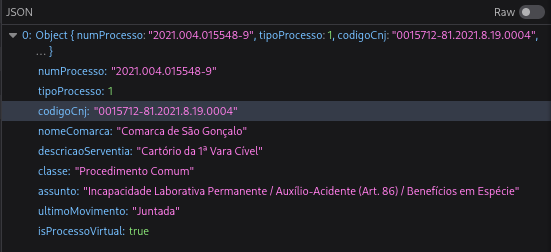
\includegraphics[keepaspectratio,width=1\textwidth]{img/tj-rj-ww3-resposta-unica-campos}
            \end{center}
        \end{column}
        \begin{column}{0.5\textwidth}
            \begin{center}
                Numeração antiga:
                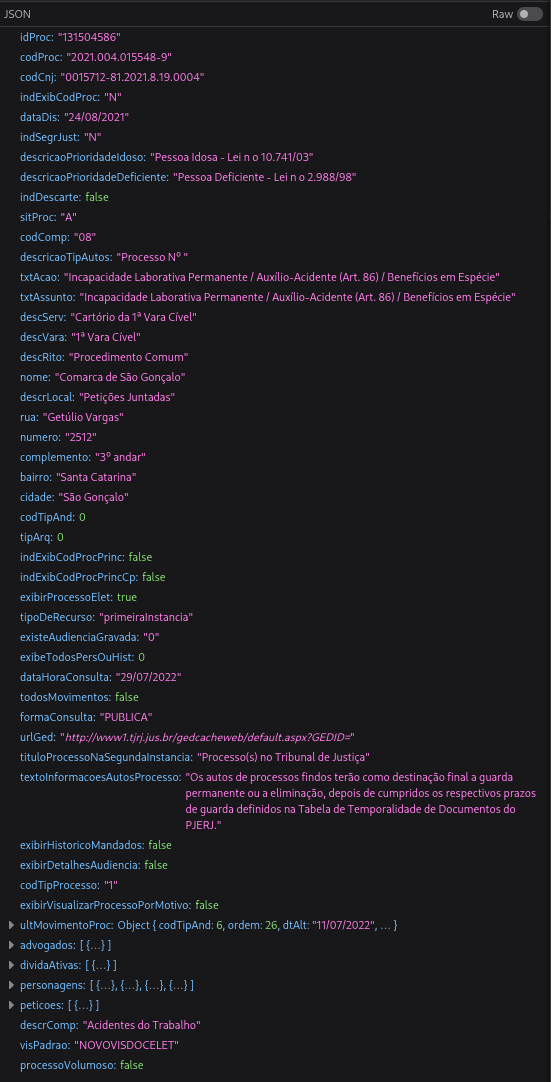
\includegraphics[keepaspectratio,height=0.7\textheight]{img/tj-rj-ww3-resposta-antiga-campos}
            \end{center}
        \end{column}
    \end{columns}
\end{frame}

\begin{frame}{Etapas}
    \begin{itemize}
        \item Descoberta de processos via numeração \textbf{unificada};
        \item \textit{Download} de processos via numeração \textbf{antiga};
        \item Seleção dos campos desejados;
        \item Exportação de processos.
    \end{itemize}
\end{frame}

\subsection{Descoberta de processos via numeração unificada}

\begin{frame}{Redução do domínio}
    Explorar o sistema de numeração para reduzir o número de entradas a serem testadas:

    \vspace{1ex}

    \begin{itemize}
        \item Obter uma lista prévia de Unidades de Origem para o TJ;
        \item Calcular os dígitos verificadores.
    \end{itemize}

    \vspace{1ex}

    Sobra apenas descobrir os valores para \texttt{NNNNNNN} até o último
    processo registrado.
\end{frame}

\begin{frame}{Processo de descoberta}
    \begin{tikzpicture}[
            node distance=2cm,
            auto,
            scale=0.6,
            transform shape,
        ]
        \node [cloud] (params) {Intervalo $I$, Ano, TJ};
        \node [block, right=1cm of params] (select-n) {Selecionar um $N \in I$};
        \node [block, right=1cm of select-n] (select-o) {Selecionar um ``OOOO'' do TJ};
        \node [block, right=1cm of select-o] (calc-digits) {Calcular ``DD''};
        \node [block, right=1cm of calc-digits] (send-request) {Envio da requisição (unificada)};
        \node [decision, below=1cm of send-request] (is-valid) {Retornou um processo?};
        \node [decision, below=1cm of select-o] (has-more-o) {Há mais ``OOOO''?};
        \node [decision, below=1cm of select-n] (has-more-n) {Há mais $N \in I$?};
        \node [block, below=0.5cm of is-valid] (send-antiga) {Envio da requisição (antiga)};
        \node [block, below=0.5cm of send-antiga] (download) {Download do processo};
        \node [cloud, below=1cm of has-more-o, text width=4.5em] (not-found) {Não encontrado};
        \node [cloud, left=1cm of has-more-n] (done) {Fim da Consulta};

        \path [line] (params) -- (select-n);
        \path [line] (select-n) -- (select-o);
        \path [line] (select-o) -- (calc-digits);
        \path [line] (calc-digits) -- (send-request);
        \path [line] (send-request) -- (is-valid);

        \path [line, dashed] (is-valid) -- node [near start] {Não} (has-more-o);
        \path [line, dashed] (is-valid) -- node [near start] {Sim} (send-antiga);

        \path [line, dashed] (has-more-o) -- node [near start] {Não} (not-found);
        \path [line, dashed] (has-more-o) -- node [near start] {Sim} (select-o);

        \path [line, dashed] (has-more-n) -- node [near start] {Não} (done);
        \path [line, dashed] (has-more-n) -- node [near start] {Sim} (select-n);

        \path [line] (not-found) -- (has-more-n);
        \path [line] (send-antiga) -- (download);
        \path [line] (download) -| (has-more-n);
    \end{tikzpicture}
\end{frame}

\section{Estratégias de Aceleração de Consulta}

\subsection{Requisições Assíncronas}

% TODO: Nesta seção, tentar explicar via diagramas (1) e (2)

\begin{frame}{Requisições Assíncronas}
    % Mostrar só em que ponto se colocariam e como foi implementado
    % (1) O diagrama pode ser uma cópia do que está na monografia
    Implementação via uso de \texttt{async/await}.

    \begin{figure}[H]
        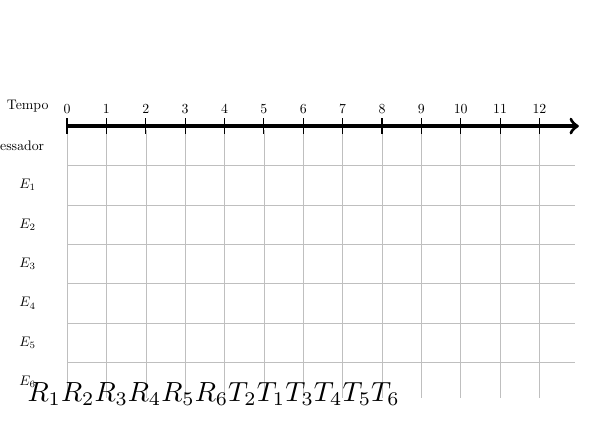
\begin{tikzpicture}[scale=0.5, transform shape]
            \useasboundingbox (0,0) rectangle (14,9.5);
            \draw[step=1cm,lightgray,very thin] (1,0.1) grid (13.9,6.9);
            \foreach \x in {0,1,2,3,4,5,6,7,8,9,10,11,12}
                \draw ((1cm+\x cm,6.8) -- (1cm+\x cm,7.2) node[anchor=south] {$\x$};
            \draw[very thick,->] (1,7) -- (14,7) node[anchor=south west] {};
            \node at (0,7.5) {Tempo};
            \node at (-0.5,6.5) {Processador};
            \foreach \i in {1,...,6}{
                \node at (0,6.5-\i) {$E_\i$};
            }
            \foreach \i in {1,2,3,4,5,6}{
                \blocoR{\i-1}{$R_\i$};
            }
            \foreach \i [count=\n] in {2,1,3,4,5,6}{
                \blocoT{\n + 5}{$T_\i$};
            }
            \blocoE{1}{1}{6}
            \blocoE{2}{2}{4}
            \blocoE{3}{3}{4}
            \blocoE{4}{4}{5}
            \blocoE{5}{5}{5}
            \blocoE{6}{6}{5}
        \end{tikzpicture}
    \end{figure}
\end{frame}

\begin{frame}{Controle de Tráfego via Lotes}
    % Comentar do uso de semáforos, etc.
    % (2) Aqui o diagrama pode ser um "zoom-out" do diagrama da monografia só
    % que com mais seções, explicitando os lotes.
    \begin{figure}[H]
        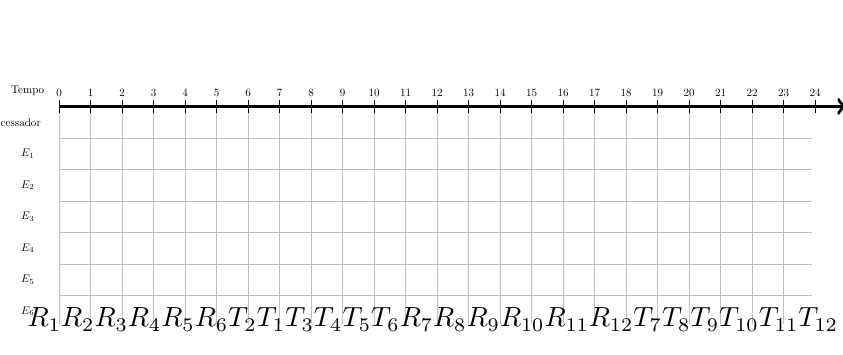
\begin{tikzpicture}[scale=0.4, transform shape]
            \useasboundingbox (0,0) rectangle (25,9.5);
            \draw[step=1cm,lightgray,very thin] (1,0.1) grid (24.9,6.9);
            \foreach \x in {0,1,2,3,4,5,6,7,8,9,10,11,12,13,14,15,16,17,18,19,20,21,22,23,24}
                \draw ((1cm+\x cm,6.8) -- (1cm+\x cm,7.2) node[anchor=south] {$\x$};
            \draw[very thick,->] (1,7) -- (26,7) node[anchor=south west] {};
            \node at (0,7.5) {Tempo};
            \node at (-0.5,6.5) {Processador};
            \foreach \i in {1,...,6}{
                \node at (0,6.5-\i) {$E_{\i}$};
            }
            \foreach \i in {1,2,3,4,5,6}{
                \blocoR{\i-1}{$R_\i$};
            }
            \foreach \i [count=\n] in {2,1,3,4,5,6}{
                \blocoT{\n + 5}{$T_\i$};
            }
            \blocoE{1}{1}{6}
            \blocoE{2}{2}{4}
            \blocoE{3}{3}{4}
            \blocoE{4}{4}{5}
            \blocoE{5}{5}{5}
            \blocoE{6}{6}{5}

            \foreach \i [count=\n] in {7,8,9,10,11,12}{
                \blocoR{\n + 11}{$R_{\i}$};
            }
            \foreach \i [count=\n] in {7,8,9,10,11,12}{
                \blocoT{\n + 17}{$T_{\i}$};
            }
            \blocoE{1}{12}{3}
            \blocoE{2}{13}{2}
            \blocoE{3}{14}{4}
            \blocoE{4}{15}{6}
            \blocoE{5}{16}{6}
            \blocoE{6}{17}{4}
        \end{tikzpicture}
    \end{figure}
\end{frame}

\begin{frame}{Controle de Tráfego via Lotes}
    \begin{enumerate}
        \item Montam-se as requisições via avaliação preguiçosa;
        \item Inicializa-se um semáforo do tamanho do lote;
        \item Itera-se pelas requisições em lotes utilizando o semáforo como
            barreira.
    \end{enumerate}
\end{frame}

\subsection{\textit{Cache} dos processos}

\begin{frame}{\textit{Cache} dos processos}
    \begin{itemize}
        \item Evita retrabalho em consultas subsequentes;
        \item Implementada como um banco de dados SQLite;
        \item Rotinas de filtragem implementadas em Python.
    \end{itemize}

    \begin{table}[H]
        \centering
        \small
        \begin{tabular}{ll}
            \toprule
            \multicolumn{2}{c}{Processos} \\
            \midrule
            Coluna & Tipo \\
            \midrule \\
            *\texttt{id} & text \\
            \texttt{cache\_state} & text \\
            \texttt{assunto} & text \\
            \texttt{json} & text \\
            \bottomrule
        \end{tabular}
    \end{table}
\end{frame}

\section{Análise de Experimentos}

\subsection{Configuração Experimental}

\begin{frame}{Configuração Experimental}
    \begin{table}[htb]
      \centering
      \begin{tabular}{ll}
        \toprule
        Parâmetro & Valores \\
        \midrule
        Número inicial do intervalo & 15712 \\
        Tamanho do intervalo & 10, 50, 100, 1000 \\
        Tamanho do lote & 1, 10, 100, 500, 1000 \\
        \bottomrule
      \end{tabular}
    \end{table}
\end{frame}

\subsection{Resultados Experimentais}

\begin{frame}[fragile]{Eficiência de requisições assíncronas}
    \begin{figure}[htb]
        \sffamily
        \centering
        \begin{tikzpicture}[scale=0.8, transform shape]
            \pgfplotstableread{io_stats-async-sync.csv}{\table}
            \pgfplotstablegetcolsof{\table}
            \pgfmathtruncatemacro\numberofcols{\pgfplotsretval-1}
            \pgfplotstablegetcolumnnamebyindex{0}\of{\table}\to{\colprincipal}
            \begin{axis}[
                ybar,
                enlarge x limits=0.15,
                symbolic x coords={
                  10, 50, 100, 1000,
                },
                xtick=data,
                xticklabels from table={\table}{\colprincipal},
                ylabel={Tempo (s)},
                xlabel={Nº de processos},
                legend cell align=left,
                legend style={
                    legend pos=outer north east,
                    cells={align=left},
                },
                width=0.7\textwidth,
                height=14em,
                clip=false,
            ]
                \pgfplotsinvokeforeach{1,...,\numberofcols}{
                    \pgfplotstablegetcolumnnamebyindex{#1}\of{\table}\to{\colname}
                    \addplot table [y index=#1] {\table};
                    \addlegendentryexpanded{\colname}
                }
            \end{axis}
        \end{tikzpicture}
    \end{figure}
\end{frame}

\begin{frame}{Sync vs Async}
    \begin{table}[htb]
      \centering
      \begin{tabular}{lllll}
        \toprule
         & \multicolumn{2}{c}{Sync} & \multicolumn{2}{c}{Async} \\
        Nº de processos & IO de Rede & CPU & IO de Rede & CPU \\
        \midrule
        10 & 0.1850 & 0.0039 & 0.0158 & 0.0020 \\
        50 & 0.2386 & 0.0104 & 0.0022 & 0.0026 \\
        100 & 0.2021 & 0.0106 & 0.0012 & 0.0030 \\
        1000 & 0.2272 & 0.0061 & 0.0008 & 0.0032 \\
        \bottomrule
      \end{tabular}
    \end{table}
\end{frame}

\begin{frame}[fragile]{Tamanho de Lote}
    \begin{figure}[htb]
        \centering
        \begin{tikzpicture}[scale=0.8, transform shape]
            \pgfplotstableread{io_stats-batch-size.csv}{\table}
            \pgfplotstablegetcolsof{\table}
            \pgfmathtruncatemacro\numberofcols{\pgfplotsretval-1}
            \pgfplotstablegetcolumnnamebyindex{0}\of{\table}\to{\colprincipal}
            \begin{axis}[
                ybar,
                enlarge x limits=0.15,
                symbolic x coords={
                    10, 100, 500, 1000
                },
                ylabel={Tempo (s)},
                xlabel={Tamanho do lote},
                legend cell align=left,
                legend style={
                    legend pos=outer north east,
                    cells={align=left},
                },
                xtick=data,
                xticklabels from table={\table}{\colprincipal},
                width=0.7\textwidth,
                clip=false,
            ]
                \pgfplotsinvokeforeach{1,...,\numberofcols}{
                    \pgfplotstablegetcolumnnamebyindex{#1}\of{\table}\to{\colname}
                    \addplot table [y index=#1] {\table};
                    \addlegendentryexpanded{\colname}
                }
            \end{axis}
        \end{tikzpicture}
    \end{figure}
\end{frame}

\begin{frame}[fragile]{Tamanho de Lote: 10000 processos}
    \begin{figure}[htb]
        \centering
        \begin{tikzpicture}[scale=0.8, transform shape]
            \pgfplotstableread{io_stats-batch-size-10000.csv}{\table}
            \pgfplotstablegetcolsof{\table}
            \pgfmathtruncatemacro\numberofcols{\pgfplotsretval-1}
            \pgfplotstablegetcolumnnamebyindex{0}\of{\table}\to{\colprincipal}
            \begin{axis}[
                ybar,
                enlarge x limits=0.15,
                symbolic x coords={
                    100, 500, 1000
                },
                bar shift=-0.5em,
                ylabel={Tempo total (s)},
                xlabel={Tamanho do lote},
                axis y line*=left,
                xtick=data,
                ymin=0,
                xticklabels from table={\table}{\colprincipal},
                width=0.7\textwidth,
                height=14em,
                clip=false,
                %legend style={at={(1,1)},anchor=north west},
                legend style={at={(0,1.1)},anchor=south west},
            ]
                \pgfplotsinvokeforeach{1,...,\numberofcols}{
                    \pgfplotstablegetcolumnnamebyindex{#1}\of{\table}\to{\colname}
                    \addplot table [y index=#1] {\table};
                    \legend{Tempo total};
                }
            \end{axis}
            \begin{axis}[
                ybar,
                enlarge x limits=0.15,
                symbolic x coords={
                    100, 500, 1000
                },
                bar shift=0.5em,
                axis y line*=right,
                ylabel={Tempo (IO de Rede) (s)},
                xlabel={Tamanho do lote},
                xtick=data,
                ymin=0,
                xticklabels from table={\table}{\colprincipal},
                width=0.7\textwidth,
                height=14em,
                clip=false,
                legend style={at={(1,1.1)},anchor=south east},
            ]
              \addplot [
                red,
                fill=red!35,
              ] coordinates {
                (100, 1.27)
                (500, 1.02)
                (1000, 4.47)
              };
              \legend{Tempo de espera por IO de Rede};
            \end{axis}
        \end{tikzpicture}
    \end{figure}
\end{frame}


\begin{frame}{Eficiência da \textit{Cache}}
    \begin{table}[htb]
        \small
        \begin{tabular}{ll}
            \toprule
            Nome do intervalo & Intervalo \\
            \midrule
            $I_1$ & $[15712, 16712]$ \\
            $I_2$ & $[16212, 17212]$ \\
            $I_3$ & $I_1 \cup I_2$ \\
            \bottomrule
        \end{tabular}
        \begin{tabular}{cp{0.8\textwidth}}
            \toprule
            Cenário & Consultas \\
            \midrule
            A
            &
            $A_1$: intervalo $I_1$; $A_2$ intervalo $I_2$.
            \\
            B & Uma única consulta no intervalo $I_2$.
            \\
            C
            &
            $C_1$: intervalo $I_3$; $C_2$: intervalo $I_3$.
            \\
            \bottomrule
        \end{tabular}
    \end{table}
\end{frame}


\begin{frame}{Eficiência da \textit{Cache}}
    \begin{figure}[htb]
        \centering
        \begin{tikzpicture}[scale=0.8, transform shape]
            \pgfplotstableread{io_stats-cache-effect.csv}{\table}
            \pgfplotstablegetcolsof{\table}
            \pgfmathtruncatemacro\numberofcols{\pgfplotsretval-1}
            \pgfplotstablegetcolumnnamebyindex{0}\of{\table}\to{\colprincipal}
            \begin{axis}[
                ybar,
                bar shift=-0.5em,
                enlarge x limits=0.15,
                symbolic x coords={
                    A1, A2, B, C1, C2,
                },
                axis y line*=left,
                ylabel={Tempo total (s)},
                xlabel={Consulta},
                legend cell align=left,
                legend style={
                  at={(0,1.1)},
                  anchor=south west,
                },
                xtick=data,
                xticklabels from table={\table}{\colprincipal},
                ymin=0,
                width=0.7\textwidth,
                clip=false,
            ]
                \pgfplotstablegetcolumnnamebyindex{1}\of{\table}\to{\colname}
                \addplot table [y index=1] {\table};
                \addlegendentryexpanded{\colname}
            \end{axis}
            \begin{axis}[
                ybar,
                bar shift=0.5em,
                enlarge x limits=0.15,
                symbolic x coords={
                    A1, A2, B, C1, C2,
                },
                axis y line*=right,
                ylabel={Tempo de espera por IO de Rede (s)},
                legend cell align=left,
                legend style={
                  at={(1,1.1)},
                  anchor=south east,
                },
                xtick=data,
                xticklabels from table={\table}{\colprincipal},
                ymin=0,
                width=0.7\textwidth,
                clip=false,
            ]
                \pgfplotstablegetcolumnnamebyindex{2}\of{\table}\to{\colname}
                \addplot [red, fill=red!35] table [y index=2] {\table};
                \addlegendentryexpanded{\colname}
            \end{axis}
        \end{tikzpicture}
    \end{figure}
\end{frame}

\section{Conclusões e Perspectivas}

\begin{frame}{Conclusões do Trabalho}
    \begin{itemize}
        \item As técnicas se mostraram eficientes;
        \item Novo gargalo: otimização da \textit{cache};
        \item Async/Await permitiu otimizações sem a complexidade de
            \textit{threads};
        \item Prova de conceito para todo TJ: extração HTML;
        \item A ferramenta se torna capaz de colaborar com Jornalistas
            Investigativos.
    \end{itemize}
\end{frame}

\begin{frame}{Conclusões adicionais}
    \begin{itemize}
        \item Twisted se mostrou uma barreira para testagem;
        \item Decisões arquiteturais do TJ-RJ impactaram e viabilizaram a
            produção;
        \item Todo o trabalho feito com ferramentas de Software Livre.
    \end{itemize}
\end{frame}

\begin{frame}{``O que fazer?''}
    % Trabalhos Futuros
    \begin{itemize}
        \item Otimizações:
            \begin{itemize}
                \item Explorar frequência conhecida de processos em unidades de origem;
                \item Buscas no banco de dados puramente via SQL;
                \item Indexação de assuntos.
            \end{itemize}
        \item Melhorias de Interface:
            \begin{itemize}
                \item Não depender de intervalos de processos;
                \item Separar \textit{Download} de Consulta;
                \item Melhor distribuição dos assuntos.
            \end{itemize}
    \end{itemize}
\end{frame}

%%%
%%% Slide final
%%%
{
    \usebackgroundtemplate{
\includegraphics[width=\paperwidth]{capa.png}}
    \begin{frame}[plain]
        \vspace{15mm}
        \begin{center}
            \textcolor{cinza}{\textbf{Discussões abertas}}
        \end{center}
        \vspace{-6mm}
        \begin{center}
        \textcolor{cinza}{
            \scriptsize{E-mail: jpaulotiz@gmail.com}}
        \end{center}
        \vspace{-6mm}
        \begin{center}
        \textcolor{cinza}{\scriptsize{Telefone: (48) 99153-1404}}
        \end{center}
        \vspace{-6mm}
        \begin{center}
        \textcolor{cinza}{\scriptsize{
            Site: \url{https://github.com/jptiz}
        }}
        \end{center}
    \end{frame}
}

\end{document}

